% Appendix D, Figure D.4 --- "The icosahedral POVM, end to end".  The layout only.
%
% Layout: card_oct_body.tex's header is binding.  Deviations from it, and only
% they, are listed here.
%
%   * band 1 NESTS the worked $E_1$ under the two vertex blocks, in the slack
%     the sphere leaves beside them -- zero words, and it is what gives the
%     covariance rule $E_{g(k)} = U_g E_k U_g^\dagger$ an effect to act on.
%     It costs 0pt: the panel, not the right column, sets the row.
%   * the vertex blocks carry no effect column (twelve two-line pmatrices do
%     not fit beside a panel), which is why the worked effect is printed.
%   * band 2 runs 377pt + 75pt: the circuit is 375.032bp and the side column
%     holds $B$ and $C$ -- the two matrices that DIFFER between this card and
%     the dodecahedron's.  The unfactored $A$, which the pair shares, is the
%     chapter head's (assertion 32 refuses to write this card until it is
%     there).  Measured: A on the card costs 43.81pt.
%   * head 4 carries ", rightmost factor first": this card prints two
%     composite atlas words and the order decides the rotation (19c).
%   * band 4's protocol line carries the two-jobs sentence: a full 2T draw
%     realizes AND twirls -- Appendix F.3.3's crossing card.  Check 19d backs
%     it and keeps that phrase off the other four, which carry their own rung
%     of the same ladder.  This is the card where the coin (six words) and
%     the draw (T's twelve rotations) part company in size and not in
%     verdict, so the sentence names the DRAW and never the ray list above
%     it.
% All macros below are \def and therefore local to the figure environment.
\parindent=0pt \parskip=0pt
% Auto-generated by code/_build_povm_cards.py -- DO NOT EDIT.
% The data blocks of the icosahedral card of Appendix D
% (paper/figures/card_icos_body.tex \input's this and calls them).  Every
% number is derived from code/data/*.npz, Decker's circuits as
% randomized_decker rebuilds them, Figure 1.1's own \RecipeSeriesStrip, and
% Tables E.1, 5.2, D.1, D.3 and D.4, and is checked back against them before
% this file is written; see the builder's docstring for the checks (and
% _povm_cards_controls.py, which shows each of them failing on one corrupted
% literal: 100 negative controls, all aborting, 0 stale).
% Requires: booktabs, mathtools, hyperref, and the thesis macros \Id, \pmat,
% \bra, \ket, \braket, \Tr, \C, \sigmavec, \TwoT, \TwoO, \TwoI, \phig,
% \invphig, \sigmaz.  The body defines \NIS, \CTR, \PBOX, \COL, \FULLHEAD,
% \BANDRULE and \TAB, which \CardSide and the tables use.
% Regenerate with `cd code && uv run _build_povm_cards.py`.

\newcommand{\CTitle}{The icosahedral POVM, end to end}
\newcommand{\CPtrStrip}{Introduction reference: Figure~\ref{fig:tetrahedron-recipe}}
\newcommand{\CHeadA}{Vertices and effects, $E_k = \tfrac1V(\Id + \hat n_k \cdot \sigmavec)$.}
\newcommand{\CPtrA}{Table~\ref{tab:povm-atlas} $\cdot$ Equation~\eqref{eq:povmform}}
\newcommand{\CHeadB}{Circuit; the dashed $U_g$ is an optional prepended rotation.}
\newcommand{\CPtrB}{Section~\ref{subsec:rotated-povms} $\cdot$ Table~\ref{tab:decker-pose}}
\newcommand{\CHeadC}{Register $\to$ vertex, top wire first; --- never fires}
\newcommand{\CPtrC}{Table~\ref{tab:decker-labels} $\cdot$ Section~\ref{sec:decker:using}}
\newcommand{\CHeadD}{Coin over axes, no ancilla, $\ket0$-vertex first, rightmost factor first}
\newcommand{\CPtrD}{Table~\ref{tab:decker-vs-coin} $\cdot$ Section~\ref{subsec:randomized-implementations} $\cdot$ Table~\ref{tab:binary-icosahedral-group-2i}}

\newcommand{\CStrip}{{\footnotesize\setlength{\tabcolsep}{4pt}\renewcommand{\arraystretch}{0.88}%
\begin{tabular}{@{}c c c c l l l@{}}
\toprule
$V$ & group & anc. & dead & reorientation exact? & relabelling & \hyperref[tab:decker-vs-coin]{coin over axes}\\
\midrule
12 & $\TwoI$ & 3 & 4 & no thesis gate set & permuted & 6 axes, no $\Phi$\\
\midrule
\multicolumn{7}{@{}l@{}}{only the octahedral coin is exact --- this dilation is not (Theorem~\ref{thm:main}, Appendix~\ref{sec:decker:exactness})}\\
\bottomrule
\end{tabular}}}

\newcommand{\CardVertexBlockA}{%
\begin{tabular}{@{}r l r@{}}
\toprule
$k$ & $\hat n_k$\ $(\times\tfrac{1}{\sqrt{2+\phig}})$ & $\bra{0}E_k\ket{0}$ \\
\midrule
$1$ & $(+\phig,\,+1,\,\phantom{+}0)$ & $0.0833$ \\
$2$ & $(-\phig,\,+1,\,\phantom{+}0)$ & $0.0833$ \\
$3$ & $(+\phig,\,-1,\,\phantom{+}0)$ & $0.0833$ \\
$4$ & $(-\phig,\,-1,\,\phantom{+}0)$ & $0.0833$ \\
$5$ & $(\phantom{+}0,\,+\phig,\,+1)$ & $0.1271$ \\
$6$ & $(\phantom{+}0,\,-\phig,\,+1)$ & $0.1271$ \\
\bottomrule
\end{tabular}
}

\newcommand{\CardVertexBlockB}{%
\begin{tabular}{@{}r l r@{}}
\toprule
$k$ & $\hat n_k$\ $(\times\tfrac{1}{\sqrt{2+\phig}})$ & $\bra{0}E_k\ket{0}$ \\
\midrule
$7$ & $(\phantom{+}0,\,+\phig,\,-1)$ & $0.0395$ \\
$8$ & $(\phantom{+}0,\,-\phig,\,-1)$ & $0.0395$ \\
$9$ & $(+1,\,\phantom{+}0,\,+\phig)$ & $0.1542$ \\
$10$ & $(-1,\,\phantom{+}0,\,+\phig)$ & $0.1542$ \\
$11$ & $(+1,\,\phantom{+}0,\,-\phig)$ & $0.0124$ \\
$12$ & $(-1,\,\phantom{+}0,\,-\phig)$ & $0.0124$ \\
\bottomrule
\end{tabular}
}

\newcommand{\CIdent}{$\sum_k E_k = \Id$, $\Tr E_k = \tfrac16$, rank one, a $5$-design; numbered at each axis's near vertex.}
\newcommand{\CIdentB}{$E_1 = \tfrac1{12}\pmat{1 & \dfrac{\phig-i}{\sqrt{2+\phig}} \\ \dfrac{\phig+i}{\sqrt{2+\phig}} & 1}$, $E_{g(k)} = U_g E_k U_g^\dagger$.}

\newcommand{\CParams}{$U_R = R_{\hat y}(\arccos(1/(\phig\sqrt3)))$ inverts Table~\ref{tab:decker-pose}'s $R$; a drawn $U_g$ twirls and relabels outcomes by $g^{-1}$.\par\vskip1pt $A^\dagger$: Equation~\eqref{eq:adagger}; $A$: Equation~\eqref{eq:aunfactored}\par\vskip1pt $u_\pm = \sqrt{1/2 \pm \sqrt{(2+\phig)/20}}$, $v_\pm = \mp\sqrt{1/2 \pm \invphig/(2\sqrt3)}$, each $\pm1$ in the two rotation boxes is $\pm\sqrt{1/2}$\par\vskip1pt $Q_{16}^\dagger$: the CNOT $\ket{0000}\mapsto\ket{0000}$, $\ket{0101}\mapsto\ket{0001}$; $\mathsf{F}_3^\dagger \oplus I_1$, lower two wires\par\vskip1pt $\tilde{M}_{16}^\dagger = (A^\dagger \otimes (\mathsf{F}_3^\dagger \oplus I_1))\,Q_{16}^\dagger$, the Naimark extension unitary the solid box implements}

\newcommand{\CardSide}{\CTR{\hsize}{$B = \pmat{u_- & -u_+ \\ u_+ & u_-}$}\NIS{4pt}\CTR{\hsize}{$C = \pmat{v_- & v_+ \\ v_+ & -v_-}$}}

\newcommand{\CardKey}{%
\begin{tabular}{@{}c c c c c@{}}
\toprule
& \multicolumn{4}{c}{\footnotesize lower} \\
{\footnotesize upper} & $\mathtt{00}$ & $\mathtt{01}$ & $\mathtt{10}$ & $\mathtt{11}$ \\
\midrule
$\mathtt{00}$ & 10 & 4 & 2 & --- \\
$\mathtt{01}$ & 11 & 1 & 3 & --- \\
$\mathtt{10}$ & 9 & 8 & 7 & --- \\
$\mathtt{11}$ & 12 & 5 & 6 & --- \\
\bottomrule
\end{tabular}
}

\newcommand{\CKappa}{Run $U_R$ and read the key, or skip $U_R$ and read Decker's own numbered list~\cite{decker2004quantumcircuitssinglequbit}: either way $\kappa = 1$, free. His circuit with our list, index for index, is the mismatch: $\kappa = +0.116566$; under the drawn twirl it costs a $1/\kappa^2 = 73.60\times$ premium in shots, never a bias.}

\newcommand{\CRays}{$\mathbf{F}^\dagger$~$1$,\,$4$ $\cdot$ $\mathbf{X} \mathbf{F}^\dagger$~$2$,\,$3$ $\cdot$ $\mathbf{F}$~$5$,\,$8$ $\cdot$ $\mathbf{X} \mathbf{F}$~$6$,\,$7$ $\cdot$ $\Id$~$9$,\,$12$ $\cdot$ $\mathbf{X}$~$11$,\,$10$}

\newcommand{\CCoin}{Draw one, apply it, then the alignment ($9 \mapsto \hat z$, inexact); measure $Z$. A full $\TwoT$ draw does randomness's two jobs at once: it realizes the POVM and twirls the noise (Section~\ref{sec:shadows:bills}).}

\long\def\NIS#1{\vskip #1\nointerlineskip}
\long\def\CTR#1#2{\hbox to #1{\hss #2\hss}}
\long\def\PBOX#1#2{\vtop{\hsize=#1\parindent0pt\sloppy\emergencystretch=1.5em\small #2}}
\long\def\COL#1#2{\vtop{\hsize=#1\parindent0pt\hbox{}\nointerlineskip #2}}
\long\def\FULLHEAD#1#2#3{\hbox to \hsize{\small\textbf{#1}\,#2\hfil{\footnotesize #3}}}
\def\BANDRULE{\vskip2pt\hrule height0.5pt\vskip1.5pt\nointerlineskip}
\long\def\TAB#1{{\small\renewcommand{\arraystretch}{0.88}\setlength{\tabcolsep}{3pt}#1}}
%
\vbox{\hsize\textwidth\parindent0pt
%
% --- title and the header strip: Figure 1.1's own row -----------------------
\hbox to \hsize{\large\bfseries \CTitle\hfil{\normalfont\footnotesize \CPtrStrip}}%
\NIS{5pt}%
\hbox{\CStrip}%
\BANDRULE
%
% --- band 1: the object -----------------------------------------------------
\FULLHEAD{1}{\CHeadA}{\CPtrA}%
\NIS{5pt}%
\hbox to \hsize{%
  \COL{170pt}{\CTR{170pt}{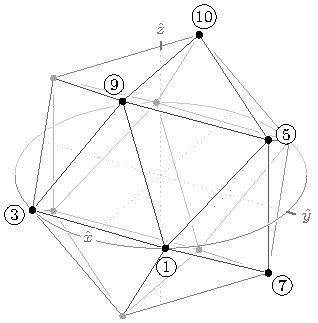
\includegraphics{figures/card_icos_sphere.pdf}}}%
  \hfil
  \COL{277pt}{\hbox to 277pt{\hfil\TAB{\CardVertexBlockA}\hskip10pt\TAB{\CardVertexBlockB}}%
    \NIS{4pt}\PBOX{277pt}{\CIdentB}}%
}%
\NIS{4pt}%
\PBOX{\hsize}{\CIdent}%
\BANDRULE
%
% --- band 2: the machine ----------------------------------------------------
\FULLHEAD{2}{\CHeadB}{\CPtrB}%
\NIS{5pt}%
\hbox to \hsize{%
  \COL{377pt}{\hbox to 377pt{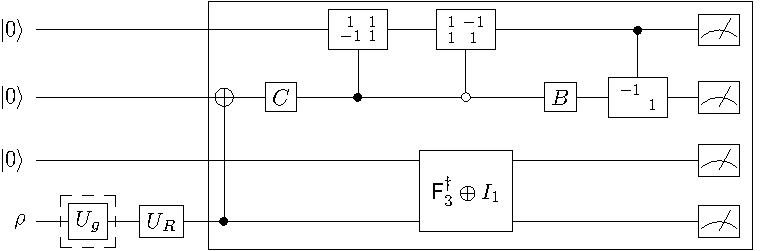
\includegraphics{figures/card_dec_icos.pdf}\hss}}%
  \hfil
  \COL{75pt}{\small\CardSide}%
}%
\NIS{5pt}%
\PBOX{\hsize}{\CParams}%
\BANDRULE
%
% --- band 3: the readout ----------------------------------------------------
\FULLHEAD{3}{\CHeadC}{\CPtrC}%
\NIS{5pt}%
\hbox to \hsize{%
  \COL{200pt}{\TAB{\CardKey}}%
  \hfil
  \COL{244pt}{\PBOX{244pt}{\CKappa}}%
}%
\BANDRULE
%
% --- band 4: the alternative ------------------------------------------------
\FULLHEAD{4}{\CHeadD}{\CPtrD}%
\NIS{5pt}%
\PBOX{\hsize}{\CRays}%
\NIS{2pt}%
\PBOX{\hsize}{\CCoin}%
}%
